%!TEX root = ../lections.tex
\begin{figure}[h!]
	\centering
	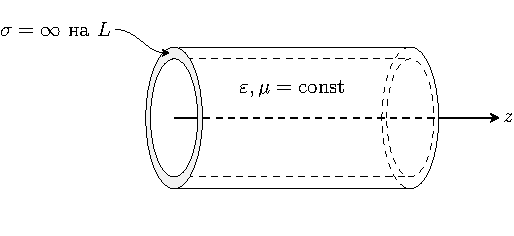
\includegraphics[scale=1.5]{img/lect2_ris1}
	\caption{Линия передачи}
	\label{fig:wavegain:1}
\end{figure}

\begin{figure}[h!]
	\centering
	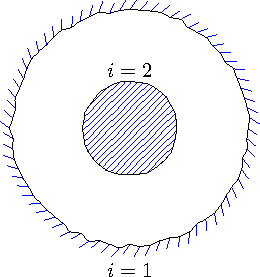
\includegraphics[scale=1.5]{img/lect2_ris2}
	\caption{Линия из разных проводников. Вид в разрезе}
	\label{fig:wavegain:2}
\end{figure}

\subsection{Математическая формулировка задачи отыскания волн в линиях передачи}

\begin{figure}[h!]
	\centering
	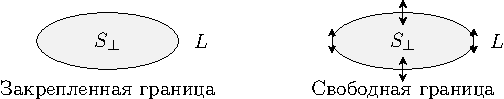
\includegraphics[scale=1.5]{img/lect2_ris3}
	\caption{Граничные условия Дирихле и Неймана в матфизике}
	\label{fig:wavegain:3}
\end{figure}

\begin{figure}[h!]
	\centering
	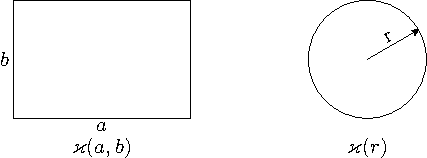
\includegraphics[scale=1.5]{img/lect2_ris4}
	\caption{Различная геометрия линии}
	\label{fig:wavegain:4}
\end{figure}

\begin{figure}[h!]
	\centering
	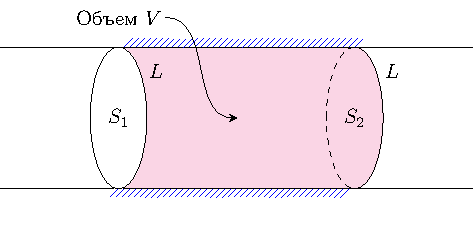
\includegraphics[scale=1.5]{img/lect2_ris5}
	\caption{Геометрия задачи}
	\label{fig:wavegain:5}
\end{figure}

\begin{figure}[h!]
	\centering
	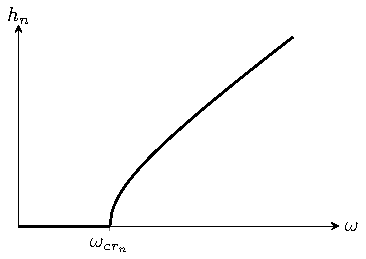
\includegraphics[scale=1.6]{img/lect2_ris6}
	\caption{Зависимость реальной части поперечного волнового числа от частоты}
	\label{fig:wavegain:5}
\end{figure}

\subsection{Дисперсионное уравнение}